\documentclass{article}
\usepackage{graphicx}
\usepackage{minted}

\begin{document}

\title{Assignment 2 - TDT4136}
\author{Ulrik Bernhardt Danielsen}

\maketitle

\begin{abstract}
Implementation of the A* best-search algorithm.
\end{abstract}

\section{How to run the code}
To run the program, insert "python assignment2.py" into your terminal. Then insert the task you want to show.
\begin{minted}{bash}
$ python assignment2.py
$ Task: 1
\end{minted}
\noindent
Now a image should appear with the solution of the chosen task. If you want to run the code in an IDE you may have to manually edit the task variable in the main function.

On the next pages the results from the tasks are presented.
\newpage

\section{Part 1}
\subsection{Task 1}

\begin{figure}[h!!!!]
	\centering
	\begin{minipage}{0.4\textwidth}
		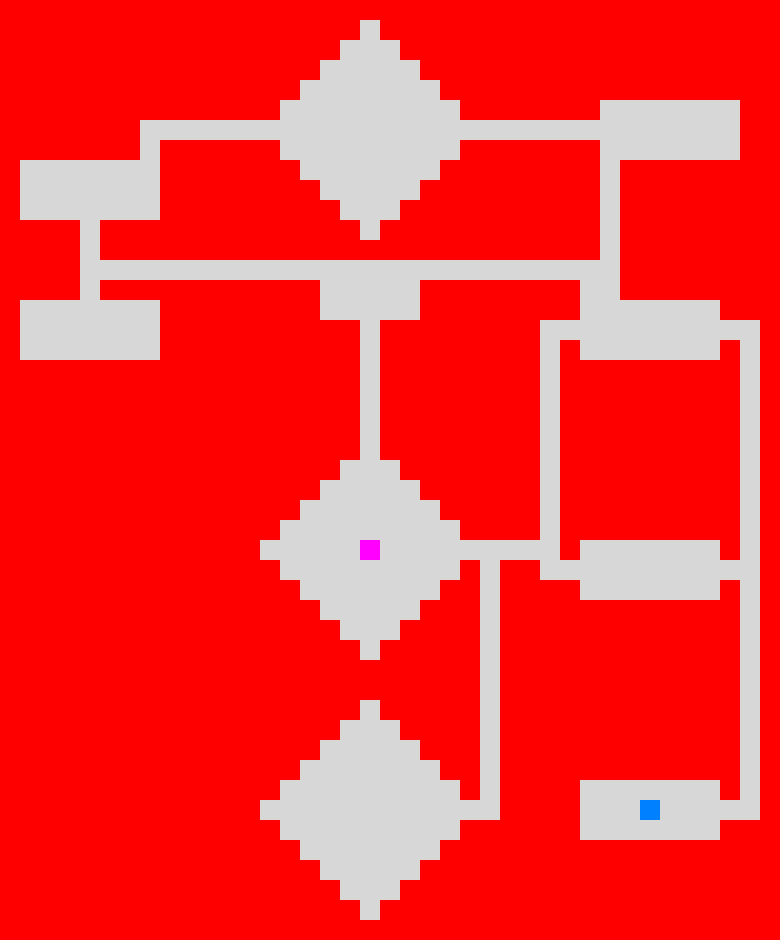
\includegraphics[width=\textwidth]{images/map1}
    		\caption{Map 1}
	\end{minipage}
	\hfill
	\begin{minipage}{0.4\textwidth}
		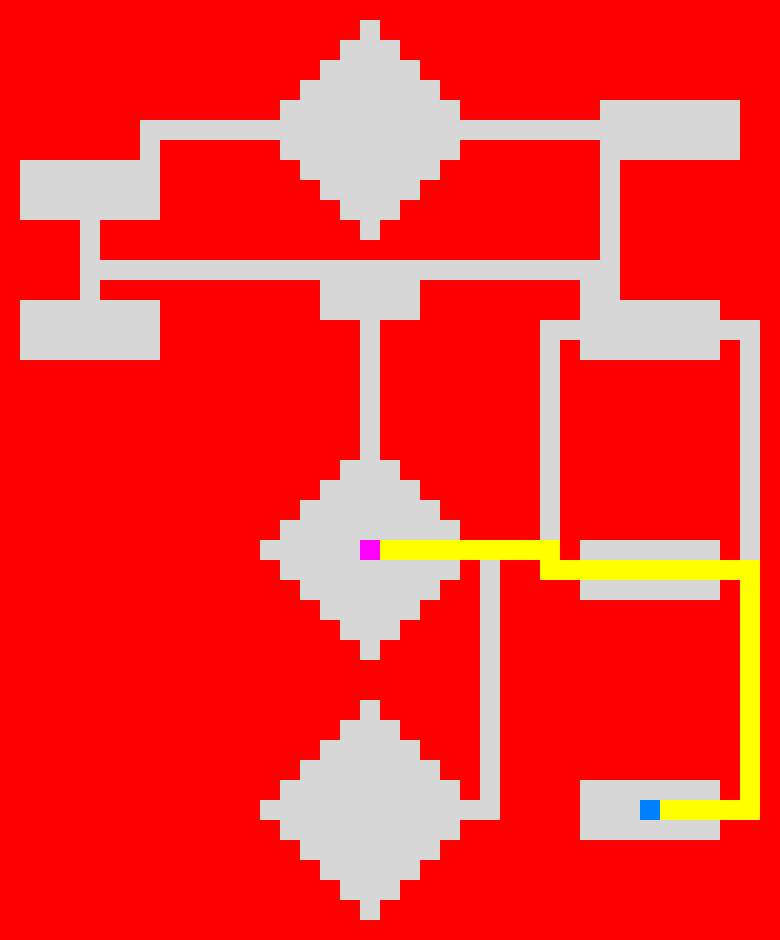
\includegraphics[width=\textwidth]{images/map1_solution}
    		\caption{Map 1 with solution}
	\end{minipage}
\end{figure}


\subsection{Task 2}
'\begin{figure}[!h]
	\centering
	\begin{minipage}{0.4\textwidth}
		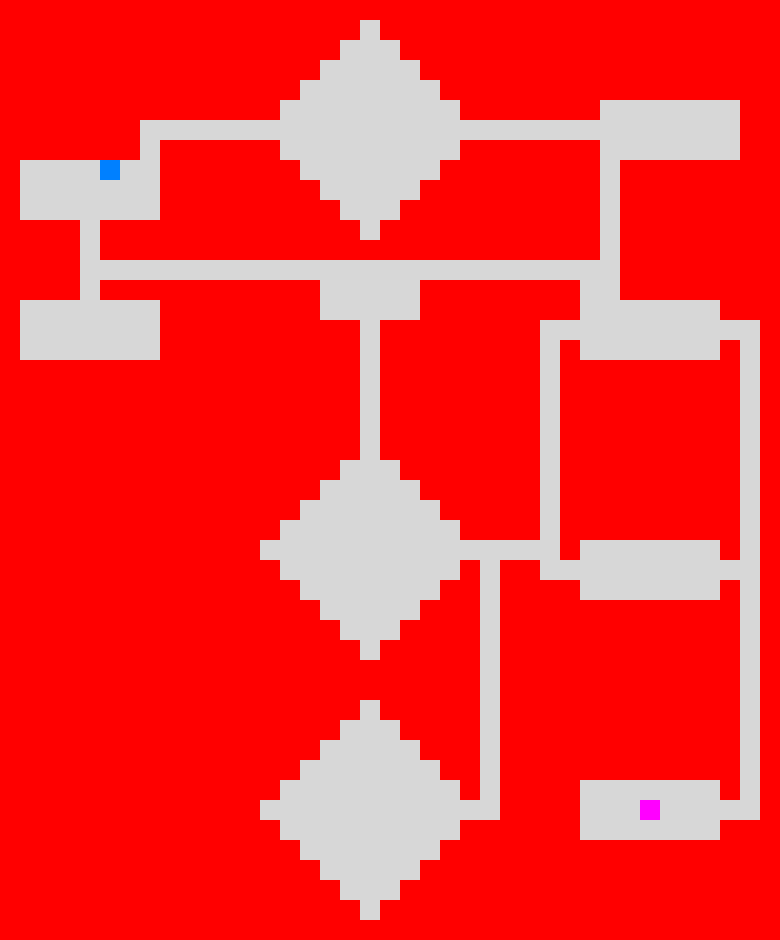
\includegraphics[width=\textwidth]{images/map2}
    		\caption{Map 2}
	\end{minipage}
	\hfill
	\begin{minipage}{0.4\textwidth}
		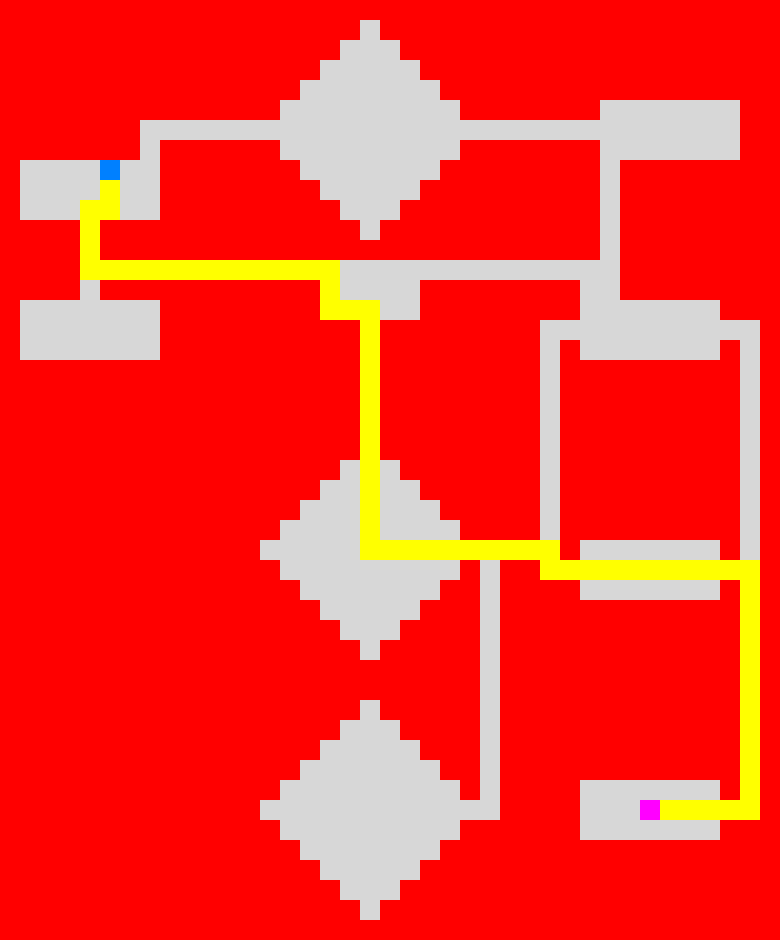
\includegraphics[width=\textwidth]{images/map2_solution}
    		\caption{Map 2 with solution}
	\end{minipage}
\end{figure}

\newpage

\section{Part 2}
\subsection{Task 3}

\begin{figure}[h]
	\centering
	\begin{minipage}{0.4\textwidth}
		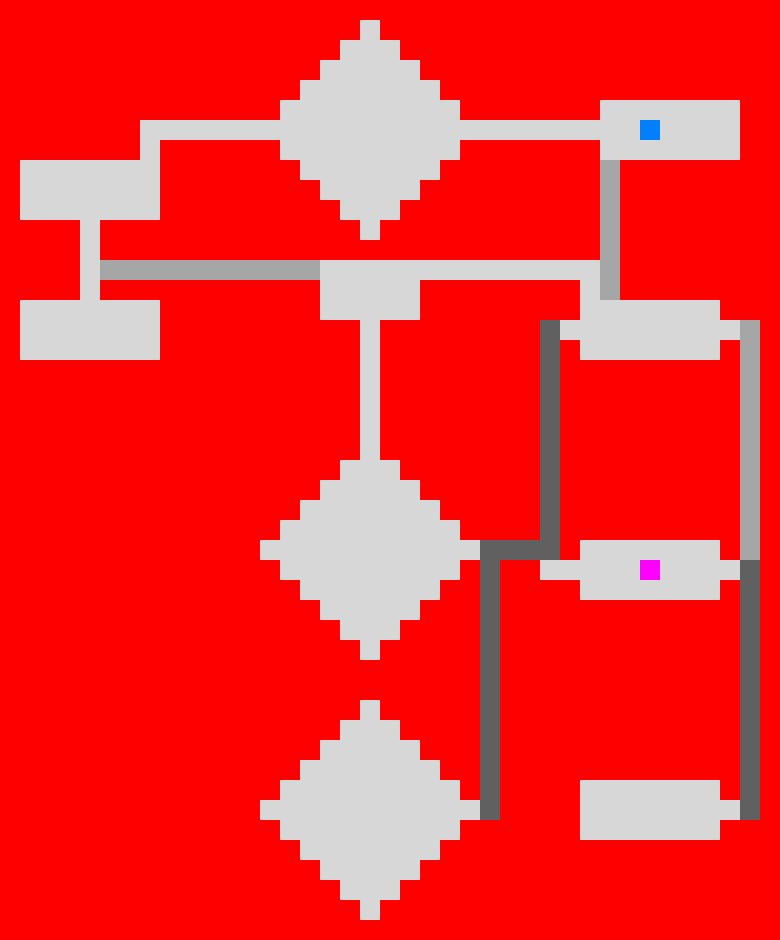
\includegraphics[width=\textwidth]{images/map3}
    		\caption{Map 3}
	\end{minipage}
	\hfill
	\begin{minipage}{0.4\textwidth}
		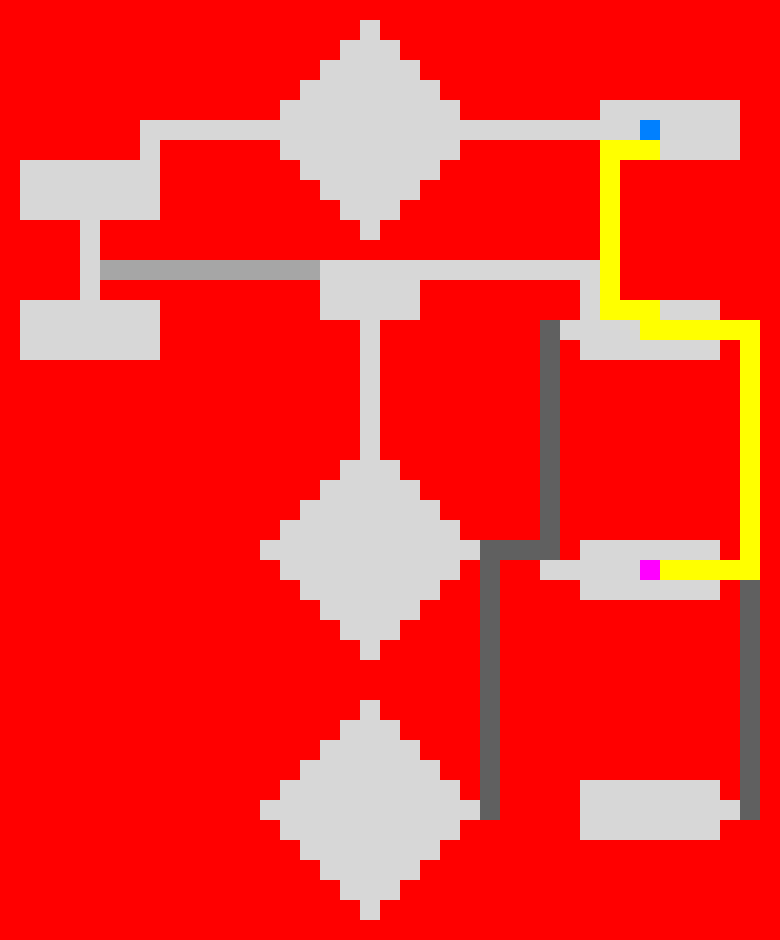
\includegraphics[width=\textwidth]{images/map3_solution}
    		\caption{Map 3 with solution}
	\end{minipage}
\end{figure}



\subsection{Task 4}
'\begin{figure}[h]
	\centering
	\begin{minipage}{0.4\textwidth}
		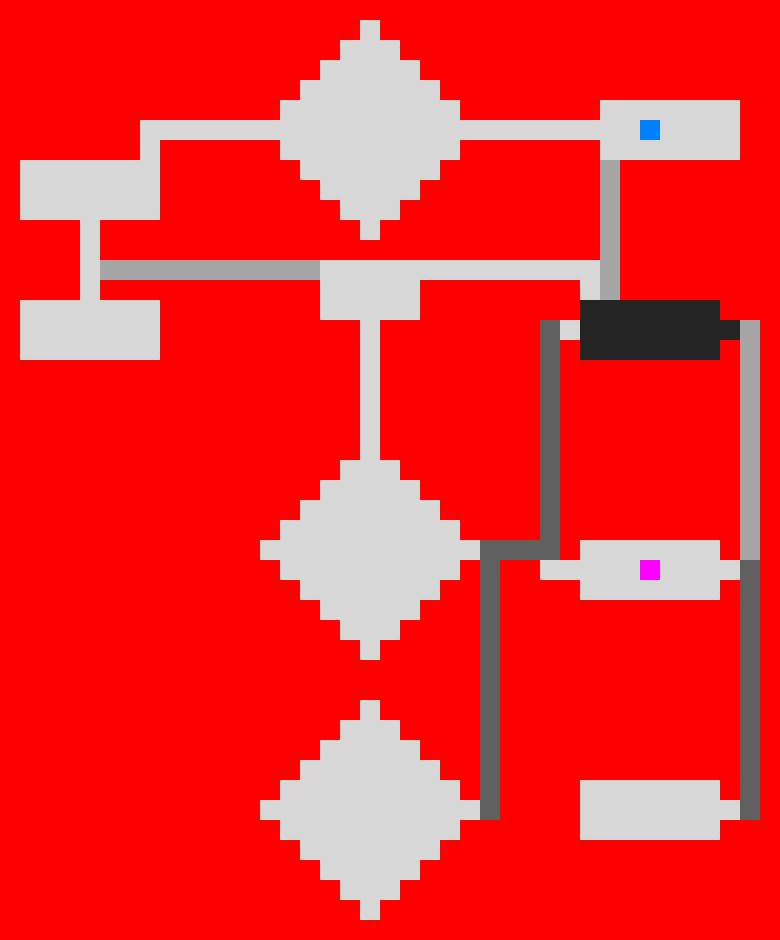
\includegraphics[width=\textwidth]{images/map4}
    		\caption{Map 4}
	\end{minipage}
	\hfill
	\begin{minipage}{0.4\textwidth}
		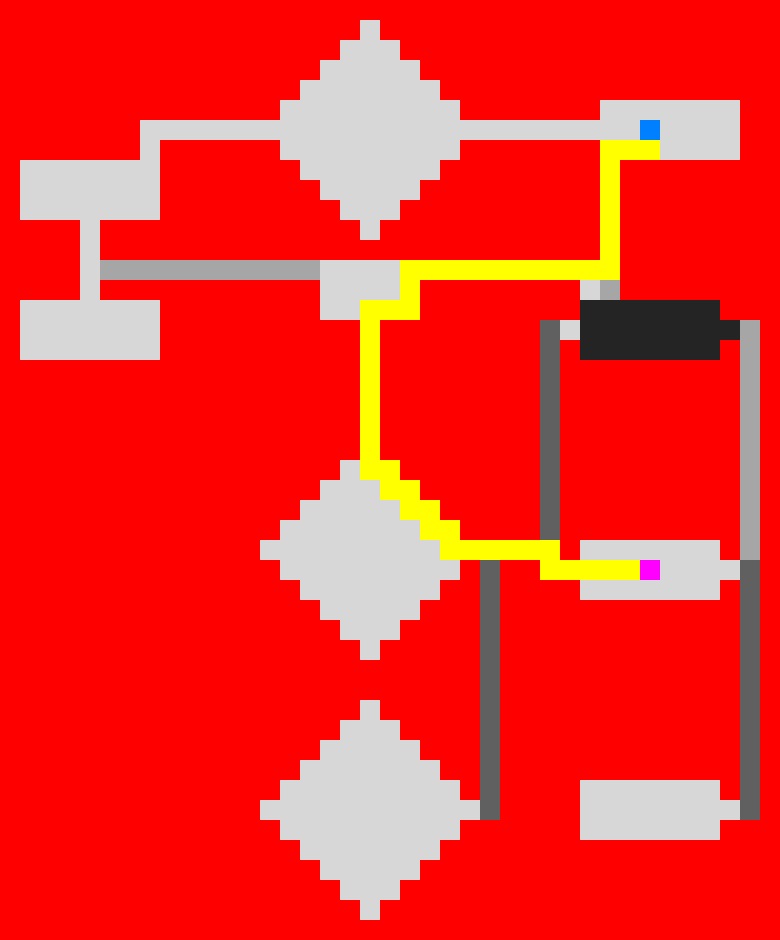
\includegraphics[width=\textwidth]{images/map4_solution}
    		\caption{Map 4 with solution}
	\end{minipage}
\end{figure}

\newpage
\section{Part 3}
\subsection{Task 5}
In this task the goal is moving left in a straight line at every fourth iteration. This means our heuristic function can be improved as we know it will be better to get to the goal quickly. Since it moves in the x-direction we have multiplied the x-part of the manhatten distance by a factor of two, as this  part is less important because it moves.
\begin{figure}[h]
	\centering
	\begin{minipage}{0.4\textwidth}
		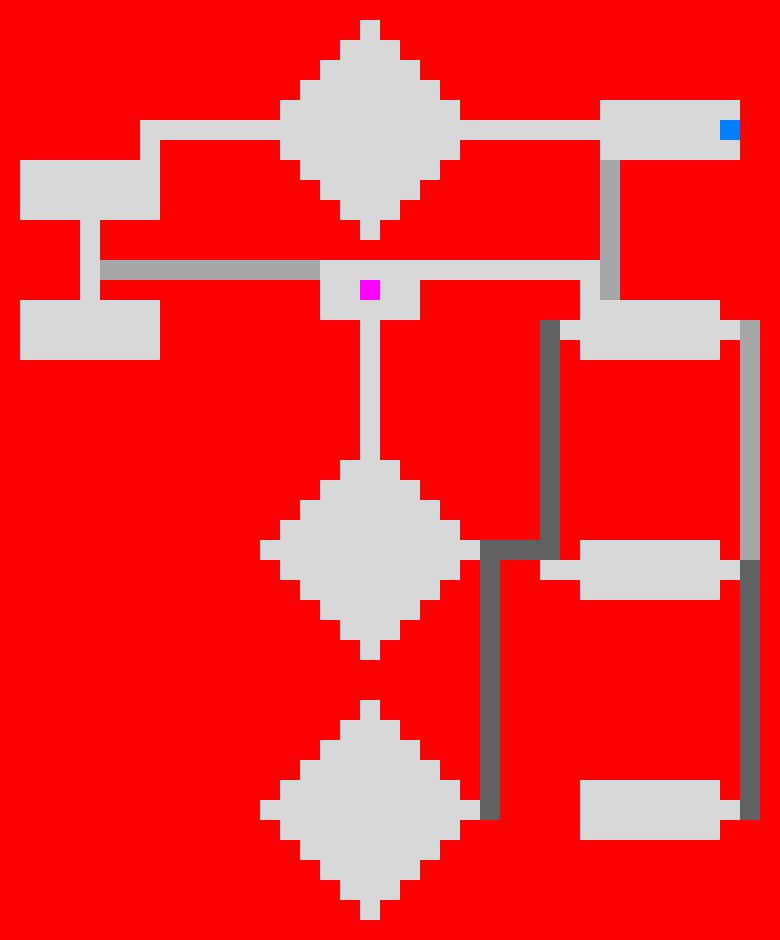
\includegraphics[width=\textwidth]{images/map5}
    		\caption{Map 5}
	\end{minipage}
	\hfill
	\begin{minipage}{0.4\textwidth}
		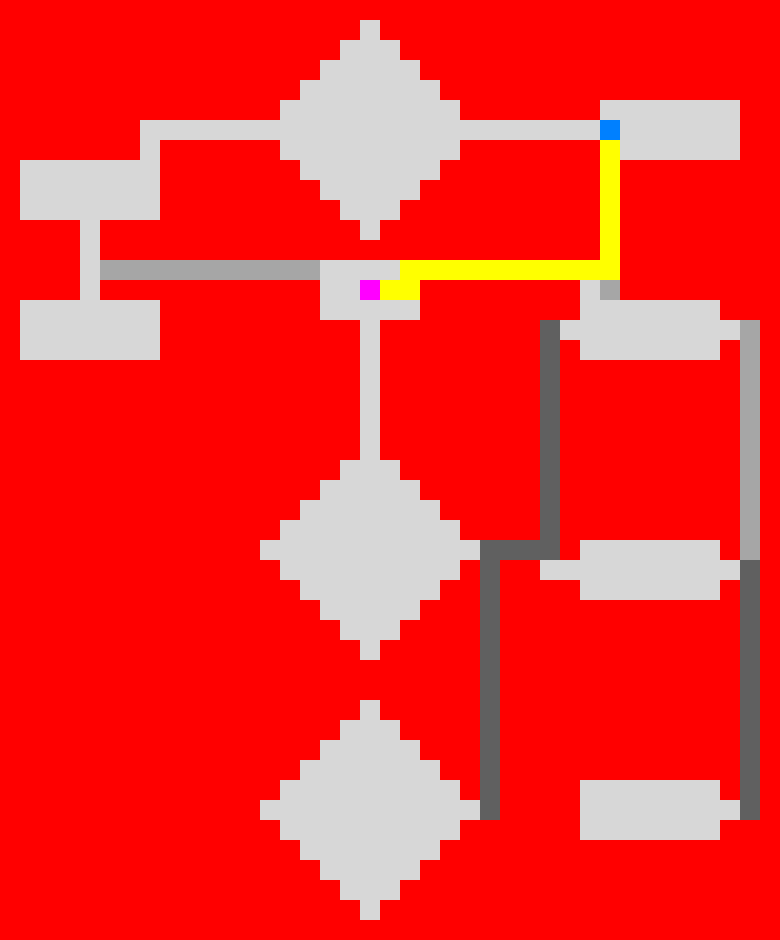
\includegraphics[width=\textwidth]{images/map5_solution}
    		\caption{Map 5 with solution}
	\end{minipage}
\end{figure}

\end{document}
